%https://www.lama.univ-savoie.fr/mediawiki/index.php/G%C3%A9n%C3%A9ration_et_r%C3%A9solution_de_labyrinthes
% https://cpge-itc.github.io/itc1/5_graph/3_traversal/labyrinth/#animation-du-dfs
\exer{Génération et parcours de labyrinthe}
%\begin{flushright}
%
%\end{flushright}
\setcounter{numques}{0}


\subsection*{Génération d'une grille}

Soit une grille rectangulaire $n\times p$ constituée de $n$ colonnes et de $p$ lignes contenant toutes les arêtes possibles. On modélise cette grille par un graphe dont l'ensemble des sommets est donné par les couples $(i,j)$ tels que $i\in\llbracket 0,n \llbracket $ et $j\in\llbracket 0,p \llbracket $. Les voisins d'un sommet $(i,j)$ sont ceux situés en haut, en bas, à droite et à gauche s'ils existent (par exemple, le sommet $(0,0)$ a comme voisin les sommets $(0,1)$ et $(1,0)$).



\begin{center}
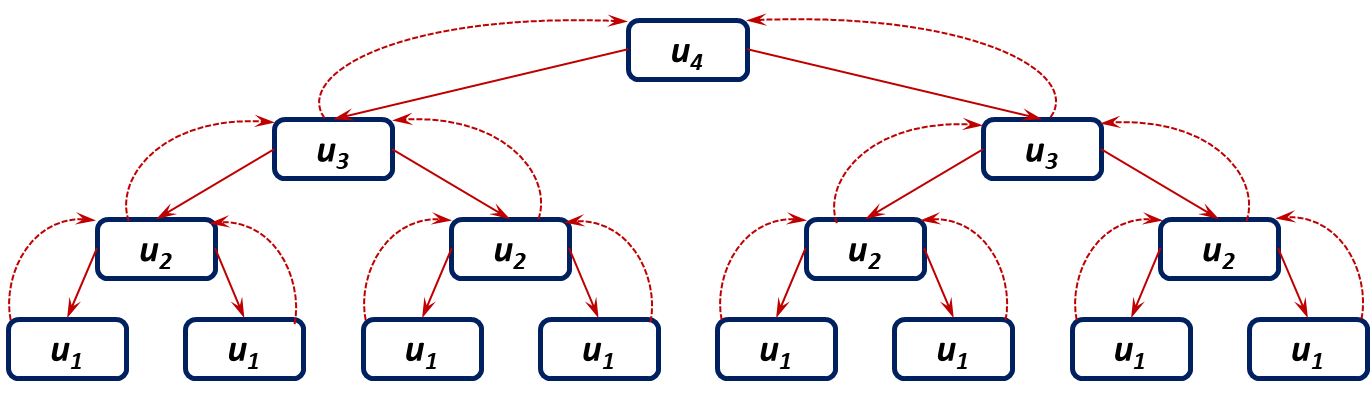
\includegraphics[width=12cm]{fig_01}
\captionof{figure}{Grille (5,3) et grille (2,2)}
\end{center}

Le graphe est implémenté par un dictionnaire d'adjacence où les clés sont les tuples, coordonnées d'un sommet. La valeur associée est une liste des sommets voisins. 


Ainsi, la grille $ 2 \times 2$ sera modélisée par le graphe suivant :

\noindent\cde{G2 = \{(0,0):[(0,1),(1,0)], (0,1):[(0,0),(1,1)], (1,0):[(0,0),(1,1)], (1,1):[(0,1),(1,0)]\}}.

\question{Écrire la fonction \cde{creer\_graphe(n:int, p:int) -> dict} permettant de créer le graphe d'une grille de \cde{n} colonnes et \cde{p} lignes.}

On souhaite afficher ce graphe en utilisant \cde{matplotlib}. Pour cela, on va commencer par tracer chacune des arêtes puis chacun des sommets. 

\question{Écrire la fonction \cde{get\_sommets(G:dict) -> (list,list)} renvoyant deux listes \cde{les\_x} et \cde{les\_y} contenant respectivement les abscisses des sommets et les ordonnées des sommets.}

\question{Écrire la fonction \cde{trace\_sommets(G:dict) -> None} qui affiche les sommets en utilisant un point rouge (\cde{`r.`}) ou cercle rouge (\cde{`ro`}).}

\question{Écrire la fonction \cde{get\_aretes(G:dict) -> list} renvoyant la liste des arêtes du graphe sous la forme d'une liste de listes de tuples. Une arête est donc une liste de sommets où les sommets sont des tuples. Les arêtes ne devront être présentes qu'une fois. }

Par exemple : \cde{get\_aretes(G2)} peut renvoyer la liste suivante : 

\cde{[[(0,0),(0,1)],[(0,0),(1,1)],[(0,1),(1,1)],[(1,0),(1,1)]]} (l'ordre des arêtes et des sommets peut être complètement différent).

\question{Écrire la fonction \cde{trace\_aretes(G:dict) -> None} qui affiche les arêtes en utilisant un trait bleu. Exemple : pour tracer l'arête [(0,2),(1,2)], il faut utiliser l'instruction \cde{plt.plot([0,1],[2,2],'b')}.}


\question{Écrire la fonction \cde{trace\_graphe(G:dict) -> None} qui permet de tracer les sommets au dessus des arêtes.}

\begin{center}
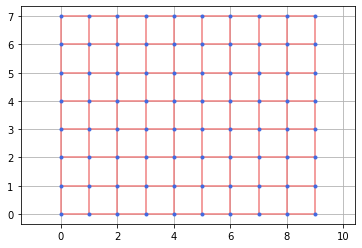
\includegraphics[width=6cm]{grille_10_8}
\captionof{figure}{Grille 10 colonnes 8 lignes}
\end{center}

\subsection*{Génération d'un labyrinthe}

Dans notre cas, résoudre le labyrinthe consiste en partir du sommet (0,0) (sommet en bas à gauche) et à se déplacer sur les arêtes dans le but d'atteindre le sommet en haut à droite. 
Pour générer un labyrinthe, nous allons réalisé un parcours de la grille \cde{G} (en largeur ou en profondeur). Le labyrinthe sera lui-même un graphe noté \cde{L}. À chaque fois qu'on découvrira un sommet à visiter, on ajoutera une arête entre le sommet père et ses voisins (s'ils ne sont pas dans le labyrinthe). 

\textbf{A REFORMULER}


\question{Écrire la fonction \cde{ajouter\_arete(G:dict, s1:tuple, s2: tuple) -> None} qui permet d'ajouter l'arête \cde([s1,s2]) au graphe \cde{G}. Il faudra vérifier que les sommets n'existent pas déjà...}

\textbf{Donner un exemple}

\question{Écrire la fonction \cde{parcours\_largeur(G:dict, s:tuple) -> dict} qui permet de créer un labyrinthe en largeur à partir d'un graphe \cde{G}. Tracer le labyrinthe obtenu.}

\question{Écrire la fonction \cde{parcours\_profondeur(G:dict, s:tuple) -> dict} qui permet de créer un labyrinthe en profondeur à partir d'un graphe \cde{G}. Tracer le labyrinthe obtenu.}

\begin{center}
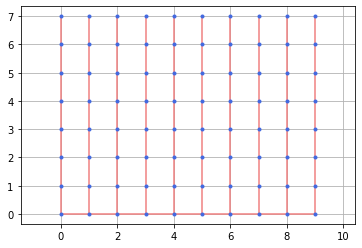
\includegraphics[width=6cm]{grille_10_8_largeur.png}
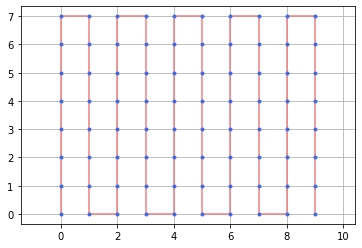
\includegraphics[width=6cm]{grille_10_8_profondeur.png}
\captionof{figure}{Labyrinthes en largeur et en profondeur}
\end{center}

Comme vous pouvez le constater, le coté aléatoire de ces labyrinthes est discutable :).
Il est possible de mélanger une liste en utilisant le module \cde{random} : \cde{random.shuffle(voisins)} permet de mélanger la liste de tuples \cde{voisins}.

\question{Écrire les fonctions \cde{labyrinthe\_largeur(G:dict, s:tuple) -> dict} et \cde{labyrinthe\_profondeur(G:dict, s:tuple) -> dict} permettant de prendre cette remarque en compte. Quelle fonction permet d'obtenir un labyrinthe acceptable ?}

\begin{center}
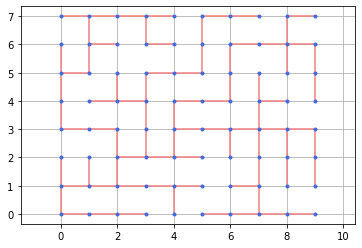
\includegraphics[width=6cm]{labyrinthe_10_8_profondeur.png}
\captionof{figure}{Labyrinthe 10x8}
\end{center}


\subsection*{Résolution d'un labyrinthe}

Il est possible de résoudre le labyrinthe en utilisant un parcours en largeur ou un parcours en profondeur. 

\question{Écrire la fonction \cde{resolution\_largeur(G:dict, s:tuple) -> list} qui permet de résoudre le labyrinthe en utilisant un parcours en largeur. Cette fonction renvoie la liste des sommets permettant d'atteindre le sommet en haut à droite depuis le sommet en bas à gauche.}

\question{Afficher en trait épais noir la solution donnée par le parcours en largeur.}

\question{Répondre aux mêmes questions en utilisant un parcours en profondeur.}